\documentclass[20pt]{beamer}
\usepackage{amssymb,amsmath}
\usepackage{dsfont}
\usepackage{fancyvrb}  % for including files
\usepackage{empheq}
\usepackage{graphicx}
\usepackage{cancel}
\usepackage{hyperref}
\usepackage{tikz}

\hypersetup{colorlinks=true}

\DeclareMathOperator{\sgn}{sgn}

\geometry{letterpaper, landscape}

\mode<presentation>{\usetheme{Warsaw}}

\usetikzlibrary{positioning}

\title{Uplift Modeling in Algorithmic Marketing}
\date{January 4, 2022}
\author{William Wong}

\begin{document}

\begin{frame}
  \titlepage
\end{frame}



\begin{frame}{Outline}
  \begin{itemize}
  \item Introduction

  \item Review of causal inference
    % \begin{itemize}
    %   \item xx
    % \end{itemize}
  \item Three methods of modeling uplift

  \item Numerical example using CausalML
  \end{itemize}
\end{frame}


\begin{frame}{What is Uplift Modeling?}
\begin{itemize}
  \item Uplift modeling refers to the set of techniques used to model the incremental impact of an
  action or treatment on a customer outcome.

  \item It is both a causal inference problem and a machine learning one.

  \item There are 100 customers belonging to 4 segments as shown in the figure below.
\end{itemize}

  \begin{figure}[p]
    \centering
    \includegraphics[width=6in]{./images/customer_segments.png}
    %\caption{The Four Customer Segments}
  \end{figure}

\end{frame}



\begin{frame}{Cumulative Uplift}
  \begin{figure}[!tbp]
    \centering
    \begin{minipage}[b]{0.6\textwidth}
      \includegraphics[width=\textwidth]{./images/cumulative_uplift.png}
    \end{minipage}
    \hfill
    \begin{minipage}[b]{0.35\textwidth}
      \includegraphics[width=\textwidth]{./images/customer_segments.png}
    \end{minipage}
  \end{figure}

  \begin{itemize}
  \item In the example above, there are 100 customers who belong to the 4 separate segments.

  \item The use cases for uplift modeling:
    \begin{itemize}
    \item Target the Persuadables for promotions.

    \item Stop reaching out to those who react to the treatment negatively (e.g., the Sleeping Dogs).
    \end{itemize}
  \end{itemize}

\end{frame}


\begin{frame}{Review of Causal Inference}
  \begin{center}
  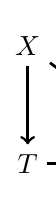
\begin{tikzpicture}[trim left=(x), trim right=(x)]
  % nodes
  \node[text centered] (t) {$T$};
  \node[right=1.5 of t, text centered] (y) {$Y$};
  \node[above = 1 of t, text centered] (x) {$X$};

  % edges
  \draw[->, line width= 1] (t) -- (y);
  \draw[->, line width= 1] (x) -- (t);
  \draw[->, line width= 1] (x) -- (y);
  \end{tikzpicture}
  \end{center}

\begin{itemize}
\item $X$ is a confounder for the treatment $T$ and the outcome $Y$.


\item $\mathbb{E}[Y^1]$ is the average value of $Y$ if \textbf{everyone was treated} with $T=1$.

\item The average treatment effect $\text{ATE} = \mathbb{E}[Y^1 - Y^0]$.

\item $\mathbb{E}[Y^1 - Y^0] \neq \mathbb{E}[Y | T=1] - \mathbb{E}[Y | T=0]$

  \begin{itemize}
    \item $\mathbb{E}[Y^1 - Y^0]$ is the \textbf{average treatment effect}, because it is comparing what would happen if the same people were treated with $T=1$ versus with $T=0$.

    \item $\mathbb{E}[Y | T=1] - \mathbb{E}[Y | T=0]$ is the \textbf{observed treatment effect}. Note that it is comparing two different populations of people.

  \end{itemize}

\item An example
  \begin{itemize}
    \item $T$ is COVID vaccination.
    \item $Y$ is mortality.
    \item $X$ is age.
  \end{itemize}

\item Consistency assumption --- the potential outcome under treatment $Y^{T=t}$ is equal to the observed outcome if the actual treatment received is $T=t$.

\item Ignorability assumption --- $\{ Y^1, Y^0\} \perp T | X$. Among subjects with the same values of $X$, we can think of treatment $T$ as being randomly assigned.

\end{itemize}
\end{frame}



\begin{frame}{Review of Causal Inference (con't)}
In a randomized trial, the distribution of $X$ will be the same in both groups since the assignment is random!

  \begin{center}
  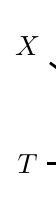
\begin{tikzpicture}[trim left=(x), trim right=(x)]
  % nodes
  \node[text centered] (t) {$T$};
  \node[right=1.5 of t, text centered] (y) {$Y$};
  \node[above = 1 of t, text centered] (x) {$X$};

  % edges
  \draw[->, line width= 1] (t) -- (y);
  %\draw[->, line width= 1] (x) -- (t);
  \draw[->, line width= 1] (x) -- (y);
  \end{tikzpicture}
  \end{center}

For observational data,

  \begin{center}
  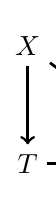
\begin{tikzpicture}[trim left=(x), trim right=(x)]
  % nodes
  \node[text centered] (t) {$T$};
  \node[right=1.5 of t, text centered] (y) {$Y$};
  \node[above = 1 of t, text centered] (x) {$X$};

  % edges
  \draw[->, line width= 1] (t) -- (y);
  \draw[->, line width= 1] (x) -- (t);
  \draw[->, line width= 1] (x) -- (y);
  \end{tikzpicture}
  \end{center}

we can match individuals in the $T=1$ group to individuals in the $T=0$ group on the covariates $X$.
\end{frame}



\begin{frame}{Problem Formulation}
  \begin{center}
  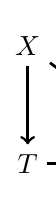
\begin{tikzpicture}[trim left=(x), trim right=(x)]
  % nodes
  \node[text centered] (t) {$T$};
  \node[right=1.5 of t, text centered] (y) {$Y$};
  \node[above = 1 of t, text centered] (x) {$X$};

  % edges
  \draw[->, line width= 1] (t) -- (y);
  \draw[->, line width= 1] (x) -- (t);
  \draw[->, line width= 1] (x) -- (y);
  \end{tikzpicture}
  \end{center}

\begin{itemize}
\item Paper by Gutierrez and G\'erardy, 2016 [\href{http://proceedings.mlr.press/v67/gutierrez17a/gutierrez17a.pdf}{link}].


\item The Conditional Average Treatment Effect for a subgroup in the population
  \begin{equation}
  \boxed{
    \text{CATE} = \tau(X) = \mathbb{E}[Y^1 | X] - \mathbb{E}[Y^0 | X] } \ ,
  \end{equation}
where $X$ is a vector of features.

  \begin{itemize}
    \item $\mathbb{E}[Y | T=t, X]$ references observed data only.

    \item $\mathbb{E}[Y | T=t, X] = \mathbb{E}[Y^{T=t} | T=t, X]$ by consistency.

    \item $\mathbb{E}[Y | T=t, X] = \mathbb{E}[Y^{T=t} | T=t, X] = \mathbb{E}[Y^{T=t} | X]$ by ignorability.
  \end{itemize}

\end{itemize}
\end{frame}

\begin{frame}{Comparison of Various Models}
\begin{table}
\begin{tabular}{|l|l|}
  \hline
  \textbf{Model} & \textbf{Prediction}  \\ \hline
  Propensity model & $\Pr(\text{buy} | T=0, X)$  \\ \hline
  Churn model & $\Pr(\text{churn} | T=0, X)$  \\ \hline
  Response model & $\Pr(\text{buy} | T=1, X)$  \\ \hline
  Uplift model & $\Pr(\text{buy} | T=1, X) - \Pr(\text{buy} | T=0, X)$  \\ \hline
  Style-affinity model & $\Pr(\text{style}=s | \text{buy}, X)$ \\ \hline
  Price-affinity model & $\Pr(\text{price}=p | \text{buy}, X)$ \\ \hline
\end{tabular}
\end{table}

\end{frame}



\begin{frame}{Method 1 --- Build Two Separate ML Models}

  \begin{itemize}
    \item Estimate $E[Y^1 | X]$ and $E[Y^0 | X]$ using the treatment group data and the control group data separately.
  \end{itemize}

\end{frame}



\begin{frame}{Method 2 --- Class Transformation}

  \begin{itemize}
    \item Define a new outcome variable $Y^* = Y^1 \frac{T}{\Pr(T=1 | X)} - Y^0 \frac{1-T}{1 - \Pr(T=1 | X)}$.

    \item Can show that $\mathbb{E}[Y^* | X] = \text{CATE} = \tau(X)$.

    \item Build a model to estimate $\mathbb{E}[Y^* | X]$.
  \end{itemize}


\end{frame}



\begin{frame}{Method 3 --- Direct Modeling using a Decision Tree}
  \begin{figure}[p]
  \centering
  \includegraphics[width=3in]{./images/decision_tree.png}
  \end{figure}

\begin{itemize}
  \item \textbf{Modify}(!) existing ML algorithms to model the uplift.

  \item There are 8 data points in a given tree node, with 4 instances in the treatment group and 4 instances in the holdout. Three out of the 4 customers in the treatment group converted (green circles), and 2 out of the 4 customers in the holdout group converted (red circles).

  \item For the best split at a given node in the tree, we want to maximize the gain of the divergence between the outcome class distributions between treatment and control [\href{https://www.aboutwayfair.com/data-science/2019/10/modeling-uplift-directly-uplift-decision-tree-with-kl-divergence-and-euclidean-distance-as-splitting-criteria/}{link}].

  \item The left child node contains the Persuadables only. Everyone in the treatment group converted, and no one in the control group converted.

  \item The right child node is just the opposite; it contains the Sleeping Dogs who generate negative value when they receive treatment.
\end{itemize}
\end{frame}



\begin{frame}{Uplift Tree and Random Forests using CausalML}
  \begin{itemize}
    \item CausalML [\href{https://readthedocs.org/projects/causalml/downloads/pdf/latest/}{link}] is an open-source Python package from Uber.

    \item Jupyter notebook [\href{https://github.com/uber/causalml/blob/master/examples/uplift_trees_with_synthetic_data.ipynb}{link}].

    \item The synthetic dataset contains columns

    \begin{itemize}
      \item {\ttfamily treatment\_group\_key}: Each row belongs to one of the \textbf{four} groups --- {\ttfamily control}, {\ttfamily treatment1}, {\ttfamily treatment2}, and {\ttfamily treatment3}. There are 1,000 rows for each group.

      \item 19 features.

      \item {\ttfamily conversion}: 0 or 1.

      %\item {\ttfamily treatment\_effect}: 0 or 1.
    \end{itemize}

    \item Uses {\ttfamily UpliftRandomForestClassifier()} as the model.

    \item CausalML has the {\ttfamily plot\_gain()} function which calculates the uplift curve given a DataFrame containing the treatment assignment, observed outcome, and the predicted treatment effect.
  \end{itemize}

\end{frame}



\end{document}
